\documentclass[times, utf8, zavrsni]{fer}
\usepackage{booktabs}
\usepackage{algorithm}
\usepackage{algorithmic}
\begin{document}

% TODO: Navedite broj rada.
\thesisnumber{4425}

% TODO: Navedite naslov rada.
\title{Alternativna tastatura za zaslone osjetljive na dodir temeljena na Fittsovom zakonu}

% TODO: Navedite vaše ime i prezime.
\author{Juraj Šušnjara}

\maketitle

% Ispis stranice s napomenom o umetanju izvornika rada. Uklonite naredbu \izvornik ako želite izbaciti tu stranicu.
\izvornik

% Dodavanje zahvale ili prazne stranice. Ako ne želite dodati zahvalu, naredbu ostavite radi prazne stranice.
\zahvala{}

\tableofcontents

\chapter{Uvod}
\section{Kratka povijest}
Tipkovnice i pisaće tehnologije postoje i razvijaju se već dosta vremena. Prvi pisaći strojevi osmišljeni su i patentirani još 1700-tih, dok su u proizvodnju krenuli 1870-tih godina. Na prvim se takvim strojevima nije čak ni mogao vidjeti onaj tekst koji se unosio jer se papir nalazio unutar njega sve do završetka stranice. Od tada su se dogodile mnoge promjene u dizajnu, načinu unošenja teksta, rasporedu tipki i samoj tehnologiji. Pisaći uređaji su s vremenom postajali sve jednostavniji i lakši za korištenje.

\begin{figure}[htb]
\centering
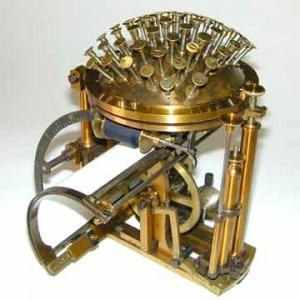
\includegraphics[width=5cm]{img/hansen.jpg}
\caption{Primjer pisaćeg stroja - Hansen writing ball (1870)}
\label{fig:hansen}
\end{figure}

Godine 1867. Cristopher Latham Sholes, uređivač novina iz Wisconsina, patentirao je svoj prvi pisaći stroj koji je razvio s prijateljima Carlos Glidden-om i Saumel W. Soule-om. Taj je stroj, kao i svi njegovi prethodnici, bio mehanički i zbog toga se već napisani znakovi nisu mogli samo tako izbrisati kao što to možemo danas na svojim računalima i mobitelima. Ukoliko je unio nešto krivo, korisnik je morao izvaditi papir i započeti iznova. Sholes je zbog toga želio osmisliti raspored znakova na tipkovnici koji bi korisniku omogućio da radi manje pogrešaka i brže unosi tekst. Prijedlog je bio da razdvoji najčešće korištene parove slova (\emph{npr. "th" u engleskom jeziku}), tako da ne budu jedno pokraj drugoga, a i da korisnik naizmjence tipka s lijevom i desnom rukom. Da bi se to ostvarilo bilo je potrebno proučiti bigrame\footnote{Frekvencija pojavljivanja parova slova u pojedinom jeziku} za određeni jezik. Sholes se mučio nekoliko godina kako bi usavršio raspored dok konačno nije došao do onog kakav se i danas koristi, a to je QWERTY.

\begin{figure}[htb]
\centering
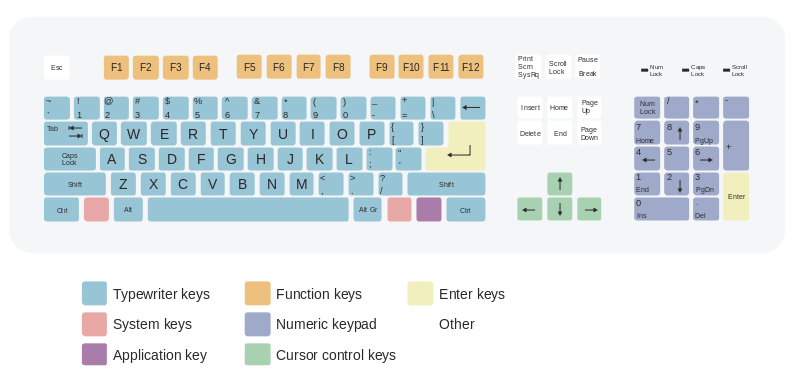
\includegraphics[width=12cm]{img/qwerty.png}
\caption{Standardni QWERTY raspored}
\label{fig:qwerty}
\end{figure}

\section{Tipkovnice danas}
Iako je QWERTY najpopularnija tipkovnica to ne znači da je i najučinkovitija. Ona se danas koristi zbog toga što su svi navikli na nju, lako je korisiti i teško je naučiti i preći na neku drugu. Postoji još mnogo različitih rasporeda i načina unošenja teksta koji su se eksperimentalno pokazali učinkovitijim od QWERTY. Navest ću neke od njih kako bi čitatelje približio tematici s kojom se bavim u ovom radu.

\begin{description}
\item[Dvorak:]
Dvorak raspodijelu tipki razvio je August Dvorak, cilj mu je bio zamjeniti QWERTY. Smatrao je da će time uvelike ubrzati i olakšati unošenje teksta jer njegova raspodijela zahtjeva manje micanje prstiju i smanjuje količinu napravljenih pogrešaka u odnosu na QWERTY. Proučavao je frekvenciju slova i fiziologiju ljudskih ruku kako bi što bolje dizajnirao svoju tipkovnicu. Iako nije uspio u naumu da Dvorak postane standardna tipkovnica, većina operacijskih sustava omogućava korisniku da je koristi. Tipkovnica je prikazana na slici \ref{fig:dvorak}.
\item[ATOMIK:]
Ova raspodijela napravljena je za korištenje stilus-a (engl. stylus) na zaslonima osjetljivim na dodir. Razvio ga je IBM koristeći Metropolis algoritam kako bi matematički minimizirali pokrete potrebne za napisati riječi na engleskom jeziku. Tipkovnica je prikazana na slici \ref{fig:atomik}.
\item[FITALY:]
Ovaj raspodijela je također napravljena za korištenje stilus-a ili jednog prsta na zaslonima osjetljivim na dodir. Najčešće korištena slova stavljena su u sredinu kako bi se minimizirali pokreti kada se tekst unosi samo jednim prstom. Tipkovnica je prikazana na slici \ref{fig:fitaly}.
\end{description}

\begin{figure}[htb]
\centering
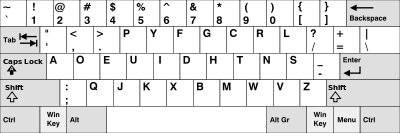
\includegraphics[width=8cm]{img/dvorak.png}
\caption{Dvorak}
\label{fig:dvorak}
\end{figure}

\begin{figure}[htb]
\centering
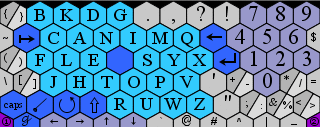
\includegraphics[width=8cm]{img/atomik.png}
\caption{ATOMIK}
\label{fig:atomik}
\end{figure}

\begin{figure}[htb]
\centering
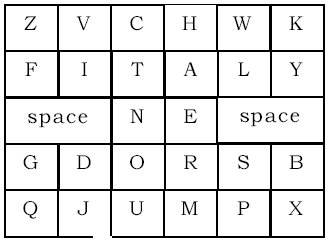
\includegraphics[width=8cm]{img/fitaly.jpg}
\caption{FITALY}
\label{fig:fitaly}
\end{figure}

\clearpage

\section{Interakcija čovjeka i računala}
Problematikom koju sam naveo u prethodna dva poglavlja bavi se područje zvano \emph{Interakcija čovjeka i računala (engl. Human-Computer Interaction)}, skraćeno \emph{HCI}. Istraživači u tom području bave se dizajnom i računalnom tehnologijom. Proučavaju se brojni načini na koje korisnik može imati interakciju s računalima te nastoji tu interakciju što više pojednostavniti, olakšati i ubrzati. Postoji mnogo načina za unos teksta, i mnogo će ih još nastati, pitanje je vremena koliko dugo će se još QWERTY koristiti. Zato je važno isprobati nove algoritme, metode i pristupe te ih eksperimentalno vrednovati kako bi se provjerila njihova učinkovitost i koliko su korisnici zadovoljni.

\chapter{Dizajniranje alternativne tipkovnice}
Ovo poglavlje obuhvaća opis samog problema te pristup njegovog rješavanja. TODO još 2-3 rečenice dodat, npr o soft keyboard, smartphonima bla bla
\section{Opis problema}
Cilj ovog rada jest osmisliti alternativnu tipkovnicu za zaslone osjetljive na dodir koristeći Fittsov zakon. Jednostavnije rečeno, radio sam na dizajniranju tipkovnice s određenim raspodijelom tipki koja bi korisniku omogućila brže unošenje teksta u odnosu na QWERTY tipkovnicu. Algoritam koji sam koristio temelji se na zasadama Fittsovog zakona (detaljnije opisan u poglavlju 2.1.1.). Taj zakon predviđa vrijeme potrebno da korisnik reagira i pomakne \emph{nešto} s jedne lokacije na drugu. To \emph{nešto} može biti npr. kursor miša, ruka, noga ili konkretno što se tiče ovog rada: prst. To vrijeme je funkcija udaljenosti do odredišne lokacije i širine te lokacije: $f(D,W)$. U okviru pronalaženja optimalne raspodijele znakova na tipkovnici, udaljenost predstavlja međusobnu udaljenost dvije tipke na tipkovnici koje planiramo uzastopno stisnuti, a širina jest širina same tipke. Kao što se već da naslutiti, cilj je minimizirati funkciju vremena što istovremeno znači i minimizirati vrijeme potrebno da se unese određeni tekst. Uzmimo kao primjer riječ PAS i da korisnik tekst unosi prstom jedne ruke. Kako bi izračunali vrijeme koje je potrebno da korisnik to unese trebamo izračunati udaljenost od P do A $d(P,A)$ i širinu od A $w(A)$, pa udaljenost od A do S $d(A,S)$ i širinu od S $w(S)$. Pretpostavlja se da je početni položaj korisnikova prsta iznad slova P, kada njega stisne potrebno je preći udaljenost $d(P,A)$ da bi se stisnula tipka A širine $w(A)$ pa udaljenost $d(A,S)$ da bi se stisnula tipka S širine $w(S)$. Iz ovoga vidimo kako će se pomoću Fittsovog zakona dobiti tipkovnica koja će imati slova koja se često uzastopno koriste, jedan blizu drugoga. Zbog toga je potrebno analizirati statistiku bigrama za ciljani jezik tipkovnice.

//TODO stavit sliku za PAS

Razmišljajući o tome kako pronaći raspodijelu tipki koja će prema Fittsovom zakonu imati najkraće vrijeme unosa teksta, pomislio sam kako bi bilo najjednostavnije isprobati svaku moguću i pronaći onu s najmanjim vremenom. Ali to nije baš tako jednostavno, ako uzmemo u obzir hrvatsku abecedu koja ima 30 slova, potrebno je ispitati $30! = 2.65*10^{32}$ mogućih različitih razmještaja, što bi vjerojatno potrajalo nekoliko stoljeća. Ako malo bolje razmislimo, ovaj problem predstavlja klasičan problem optimizacije, pitanje je kako pronaći minimum funkcije zadane Fittsovim zakonom uzevši u obzir sve moguće razmještaje slova. Postoje razne metode za rješiti taj problem, ja sam odlučio iskoristiti moć genetskog algoritma. Genetski algoritam i način na koji sam ga koristio su detaljno opisani u poglavlju 2.1.2.

\subsection{Fittsov zakon}
Fittsov zakon je opisni model ljudskog pokreta koji se primarno koristi u \emph{HCI-u}\footnote{Interakcija čovjeka i računala.} i \emph{ergonomiji}\footnote{Znanstvena disciplina koja istražuje ljudski organizam i ponašanje, te pruža podatke o prilagođenošću predmeta s kojima čovjek dolazi u kontakt.}. Kao što smo već rekli, Fittsov zakon predviđa vrijeme brzog pokreta do odredišne lokacije, to je funkcija udaljenosti do odredišta i širine tog odredišta. Ovaj zakon modelira čin pokazivanja (engl. \emph{act of pointing}), to može biti fizičko dodirivanje nekog objekta, primjerice rukom i prstom, a može biti i virtualno kao što je strelicom miša na računalu. Fittsov zakon se pokazao učinkovit u mnogo različitih slučajeva, koristeći razne dijelove tijela (ruke, noge, usne, kretanje oka...), u raznim okolinama (čak i pod vodom) i u raznim društvenim skupinama (mladi, stariji, ljudi s posebnim potrebama...). 

Ideja Fittsovog zakona prikazana je na slici \ref{fig:fitts} gdje se kao udaljenost do odredišta gleda udaljenost od dvije istaknute lokacije, a širina odredišta je širina "Take the Tour" gumba. Na slici \ref{fig:scroll} vidimo razliku između klizne trake (engl. \emph{scroll-bar}) kod OSX-a i Windows-a. Kod Windows-a su strelice za pomicanje klizne trake krajnje lijevo i krajnje desno, što više prati mentalni model osobe kojoj je to intuitivnije. S druge strane kod OSX-a su obe strelice jednu uz drugu kako bi se smanjilo vrijeme pomicanja strelice miša s jedne na drugu, što je konkretno ono čega se Fittsov zakon dotiče.

Paul Fitts je 1954. godine predložio metriku pomoću koje se vrednuje težina zadatka pokazivanja (brzog pomicanja na odredišnu lokaciju). Ta metrika se temelji na informacijskoj analogiji, gdje je $D$ udaljenost do odredišta i gleda se na njega kao na signal, a $W$ je širina ili tolerancija koja se ponaša kao šum. $ID$ predstavlja indeks težine (engl. \emph{index of difficulty}) i mjeri se u bitovima. Formula je dana izrazom \ref{eq:fitts}.
\begin{equation}
\label{eq:fitts}
ID = log_2(2D/W)
\end{equation}

Fitts je također predložio indeks izvedbe (engl. \emph{index of performance}) kao mjerilo ljudske izvedbe . Ova metrika kombinira $ID$ (\emph{index of difficulty}) s vremenom pomicanja $MT$ (\emph{movement time}) na odredišnu lokaciju. Prosječna stopa informacije koja je dobivena serijom pokreta jest prosječna informacija po pomicanju podijeljena s vremenom pomicanja. Formula je dana izrazom \ref{eq:fitts2}.
\begin{equation}
\label{eq:fitts2}
IP = ID/MT
\end{equation}
$MT$ je definiran izrazom \ref{eq:fitts3}. Parametri $a$ i $b$ koji najviše odgovaraju tom izrazu pronalaze se linearnom regresijom.
\begin{equation}
\label{eq:fitts3}
MT = a+b*ID = a+b*log_2(2D/W)
\end{equation}

\begin{figure}[htb]
  \centering
  \begin{minipage}[b]{0.45\textwidth}
    
\includegraphics[width=\textwidth]{img/fitts.png}
    \caption{Uporaba Fittsovog zakona}
    \label{fig:fitts}
  \end{minipage}
  \hfill
  \begin{minipage}[b]{0.45\textwidth}
    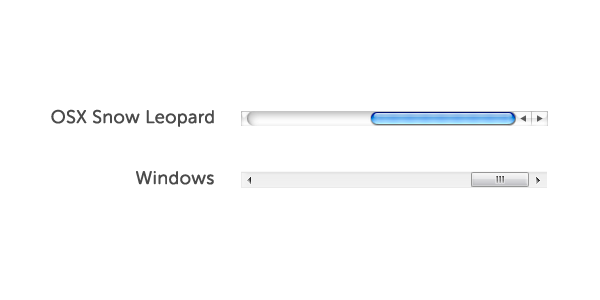
\includegraphics[width=\textwidth]{img/scroll.png}
    \caption{Uporaba Fittsovog zakona}
    \label{fig:scroll}
  \end{minipage}
\end{figure}


\subsubsection{Fittsov zakon u mom radu}
Za potrebe ovog rada koristio sam modifikaciju Fittsovog zakona kako bi mogao evaluirati pojedinu tipkovnicu. Formula je dana izrazom \ref{eq:fitts4}
\begin{equation}
\label{eq:fitts4}
t = \sum_{i=1}^{N}\sum_{j=1}^{N}\frac{P_{i,j}}{IP}log_2(\frac{D_{i,j}}{W_{i,j}} + 1)
\end{equation}
gdje je:
\begin{itemize}
\item $t$: prosječna vremenska cijena (engl. \emph{time cost})
\item $P$: matrica vjerojatnosti prelaska s jednog slova na drugu (bigrami)
\item $D$: matrica međusobne udaljenosti dva slova na tipkovnici
\item $W$: širina tipke na kojoj se nalazi određeno slovo
\item $IP$: Fittsov indeks izvedbe mjeren u bitovima po sekundi [$bit/s$]
\item $N$: broj slova u ciljanoj abecedi
\end{itemize}
Ovaj model se može pojednostavniti ako postavimo $W=IP=1$ što neće utjecati na konačne rezultate.

Opišimo sada na primjeru što izraz \ref{eq:fitts4} zapravo znači. Recimo da treba evaluirati raspored slova na tipkovnici prikazanoj na slici \ref{fig:fitts_primjer}. Prvo što nam treba je matrica vjerojatnosti $P$. Ona je dimenzija $N$x$N$ i izgleda različito za svaki jezik (za engleski jezik najveću će vrijednost imati polje koje označava bigram \emph{TH}). Nakon toga potrebno je izračunati matricu $D$. Udaljenost dva slova na tipkovnici se jednostavno računaju tako da se tipkovnica gleda kao šahovska ploča gdje svako slovo ima svoje koordinate. Primjerice udaljenost slova \emph{z} i \emph{d} je 1, a udaljenost slova \emph{ć} i \emph{h} je $\sqrt{2^2+1^2} = 2.236$. Provučemo li izračunate vrijednosti kroz izraz \ref{eq:fitts4} dobit ćemo vremensku cijenu tipkovnice koja približno iznosi $1.038$. Jedinica ove vrijednosti nam nije bitna, bitno je jedino da imamo kriterij za usporedbu dvije tipkovnice. Što je vremenska cijena tipkovnice manja to je tipkovnica "bolja". //TODO opis za 2-handed
\begin{figure}[htb]
\centering
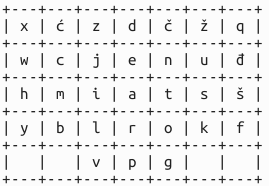
\includegraphics[width=8cm]{img/primjer.png}
\caption{Primjer tipkovnice}
\label{fig:fitts_primjer}
\end{figure}

Prethodno opisani model je preuzet je iz rada \emph{"Optimizing stylus keyboard layouts with a genetic algorithm: customization and internationalization" - Chad R. Brewbaker}.

\subsection{Genetski algoritam}
Genetski ili genetički algoritam (GA)  je heuristička metoda optimiranja koja imitira prirodni evolucijski proces. Evolucija je robustan proces pretraživanja prostora rješenja. Živa bića se tijekom evolucije prilagođavaju uvjetima u prirodi, tj. životnoj okolini. Analogija evolucije kao prirodnog procesa i genetskog algoritma kao metode optimiranja, očituje se u procesu selekcije i genetskim operatorima. Mehanizam odabira nad nekom vrstom živih bića u evolucijskom procesu čine okolina i uvjeti u prirodi. U genetskim algoritmima ključ selekcije je funkcija cilja, koja na odgovarajući način predstavlja problem koji se rješava. Slično kao što su okolina i uvjeti u prirodi ključ selekcije nad nekom vrstom živih bića, tako je i funkcija cilja ključ selekcije nad populacijom rješenja u genetskom algoritmu. Naime, u prirodi jedinka koja je najbolje prilagođena uvjetima i okolini u kojoj živi ima najveću vjerojatnost preživljavanja i parenja, a time i prenošenja svojega genetskog materijala na svoje potomke. Za genetski algoritam jedno rješenje je jedna jedinka. Selekcijom se odabiru dobre jedinke koje se prenose u slijedeću populaciju, a manipulacijom genetskog materijala stvaraju se nove jedinke. Takav ciklus selekcije, reprodukcije i manipulacije genetskim materijalom jedinki ponavlja se sve dok nije zadovoljen uvjet zaustavljanja evolucijskog procesa. Konačan rezultat je populacija jedinki (potencijalnih rješenja). Najbolja jedinka u zadnjoj iteraciji predstavlja rješenje optimiranja. Genetski algoritam izvršava se uporabom operatora križanja, mutacije, selekcije i reprodukcije. Svaki od njih objašnjen je u nastavku.

\subsubsection{Operator križanja}
U procesu križanja (engl. \emph{crossover}) sudjeluju dvije jedinke koje se nazivaju \emph{roditelji}. Dakle, križanje je binarni operator. Križanjem nastaju jedna ili dvije nove jedinke koje se nazivaju \emph{djeca}. Najvažnija karakteristika križanja jest da \emph{djeca} nasljeđuju svojstva svojih roditelja. Ako su roditelji \emph{dobri} (prošli su proces selekcije), tada će najvjerojatnije i \emph{dijete} biti dobro, ako ne i bolje od svojih roditelja. Ako jedinku predstavimo kao niz bitova onda se križanje implementira slično kao što je prikazano na slici \ref{fig:krizanje}. Bitno je napomenuti da se križanje može izvesti na mnogo različitih načina, ovisno o problemu i načinu prikaza jedinke.

\begin{figure}[htb]
\centering
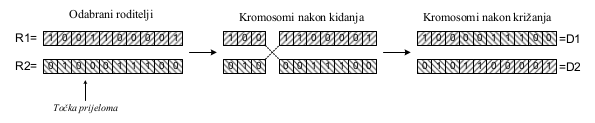
\includegraphics[width=12cm]{img/krizanje.png}
\caption{Križanje s jednom točkom prijeloma}
\label{fig:krizanje}
\end{figure}

\subsubsection{Operator mutacije}
Mutacija ili slučajna promjena jednog ili više gena je unarni operator koji djeluje nad jednom jedinkom. Rezultat mutacije je izmijenjena jedinka. Parametar koji određuje vjerojatnost mutacije $p_m$ jednog bita je ujedno i parametar algoritma. Ako vjerojatnost mutacije teži k jedinici, tada se algoritam pretvara u algoritam slučajne pretrage prostora rješenja. S druge strane, ako vjerojatnost mutacije teži k nuli, postupak će najvjerojatnije već u početku optimiranja stati u nekom lokalnom optimumu. \emph{Jednostavna mutacija} svaki bit kromosoma mijenja s jednakom vjerojatnošću $p_m$.

\begin{figure}[htb]
\centering
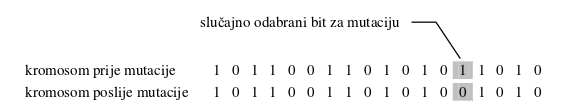
\includegraphics[width=12cm]{img/mutacija.png}
\caption{Jednostavna mutacija}
\label{fig:mutacija}
\end{figure}

\subsubsection{Operator selekcije}
Jedan od centralnih mehanizama, kako kod većine populacijskih algoritama pa i općenito, jest mehanizam \emph{selekcije}. Kod populacijskih algoritama zadaća operatora selekcije jest osigurati mehanizam koji će češće boljim rješenjima dati priliku da sudjeluju u produkciji novih rješenja, čime će se proces pretraživanja prostora rješenja voditi u područja koja više obećavaju. Postoji više različitih vrsta selekcija.

\emph{Proporcionalna selekcija} (engl. \emph{Roulette-wheel selection} funkcionira na način da sve jedinke postavimo na kolo, tako da bolja jedinka ima veću površinu na kolu (prikazano na slici \ref{fig:selekcija}). Potom zavrtimo kolo i pogledamo na kojoj se jedinki kolo zaustavilo. S obzirom da jedinki pripada to veći dio oboda kola što ima veću dobrotu, ponavljamo li eksperiment puno puta, bolje jedinke će biti češće birane od lošijih, i ta će vjerojatnost biti upravo proporionalna dobroti same jedinke.

\begin{figure}[htb]
\centering
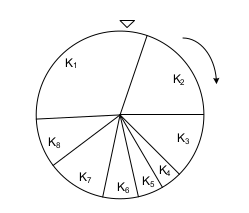
\includegraphics[width=6cm]{img/selekcija.png}
\caption{Shema genetskog algoritma}
\label{fig:selekcija}
\end{figure}

Kod \emph{k-turnirske selekcije} se iz populacije posredstvom slučajnog mehanizma odabire \emph{k} jedinki, i potom uzima najbolju. Ukoliko trebamo \emph{n} roditelja,, naprosto ćemo \emph{n} puta ponoviti turnirsku selekciju.

\subsubsection{Operator reprodukcije}
Reprodukcijom se jednostavno jedinka prenosi iz jedne generacije u drugu. Ta jedinka se odabere operatorom selekcije.

\begin{algorithm}
\caption{Genetski algoritam - pseudokod}
\label{alg:genetski}
\begin{algorithmic}
\STATE{P = stvoriPocetnuPopulaciju(VELICINA)}
\STATE{evaluiraj(P)}
\REPEAT
\STATE{novaPopulacija P' = $\emptyset$}
\WHILE{velicina(P') < VELICINA}
\STATE{odaberi R1 i R2 iz P}
\STATE{\{D1, D2\} = krizaj(R1, R2)}
\STATE{mutiraj D1, mutiraj D2}
\STATE{dodaj D1 i D2 u P'}
\ENDWHILE
\STATE{P = P'}
\UNTIL{uvjetZadovoljen}
\end{algorithmic}
\end{algorithm}

\begin{figure}[htb]
\centering
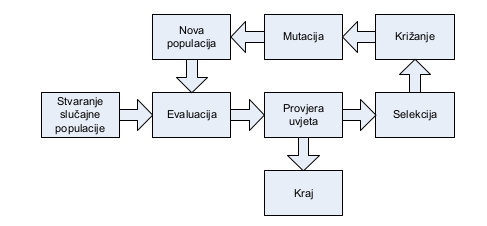
\includegraphics[width=12cm]{img/genetski_shema.png}
\caption{Shema genetskog algoritma}
\label{fig:genetski_shema}
\end{figure}

\subsubsection{Genetski algoritam u mom radu}
Jedinku u genetskom algoritmu predstavlja jedna tipkovnica sa svojim oblikom i rasporedom tipki. Jedna generacija sadrži $500$ jedinki, a $1000$ je postavljen za maksimalan broj jedinki (uvjet zaustavljanja algoritma). Algoritam koristi operatore križanja, selekcije, mutacije i reprodukcije kako bi pronašao optimalno rješenje. Tip selekcije koji se koristio jest \emph{k-turnirska selekcija} gdje je \emph{k} postavljen na $24$. Mutacija je implementirana na način da su slučajnom odabirom zamijenjene pozicije od $p\%$ znakova na tipkovnici. $p$ je postavljen na $0.3$. Križanje je napravljeno tako da su svi znakovi s pojedine tipkovnice po redu nanizani u polje. Točka prekida polja je središnji element. Nakon prekida dvije polovice se zamijene i tada nastaju 2 nova polja. Svako polje može sadržavati duple znakove. Taj problem je rješen tako da su u svakom pronađeni znakovi koji nedostaju i stavljeni umjesto duplikata. Proces križanja prikazan je na slici \ref{fig:krizanje_primjer}.

\section{Implementacija i rezultati}
TODO \\
Opisat kako sam oblikovao kod, stavit dijelove koda, opisat način na koji funkcioniraju crossover, mutation, reproduction, način na koji se pokreće program, opisat kako sam više puta pokrećao algoritam jer često zapne u lokalnom optimumu, kako sam za cost koristio 1/t, kako sam napravio varijaciju za 2-handed, opisat zašto i da želim eksperimentom provjerit rezultat ... navest sve razne layoute i rezultate koje sam dobio

U poglavlju 2.1 opisana je problematika i dobrim dijelom pristup rješavanju problema. U ovom poglavlju ćemo se detaljnije pozabaviti načinu na koji sam implementirao algoritam, rezultatima koje sam dobio i alatima koje sam koristio kako bi došao do rješenja.


\chapter{Provedba eksperimenta i obrada rezultata}

\chapter{Zaključak}
Zaključak.

\bibliography{literatura}
\bibliographystyle{fer}

\begin{sazetak}
Sažetak na hrvatskom jeziku.

\kljucnerijeci{Ključne riječi, odvojene zarezima.}
\end{sazetak}

% TODO: Navedite naslov na engleskom jeziku.
\engtitle{Alternative Touchscreen Keyboard Based on Fitts Law}
\begin{abstract}
Abstract.	

\keywords{Keywords.}
\end{abstract}

\end{document}
